%%This is a very basic article template.
%%There is just one section and two subsections.
\documentclass{article}

\usepackage[margin=2cm]{geometry}
\usepackage{multicol}

\usepackage{amsfonts}
\usepackage{amsopn}
\usepackage{amsmath}

\usepackage{hyperref}

\usepackage{graphicx}
\graphicspath{{./resources/}}

% change style of items
\newlength{\wideitemsep}
\setlength{\wideitemsep}{.5\itemsep}
\addtolength{\wideitemsep}{-7pt}
\let\olditem\item
\renewcommand{\item}{\setlength{\itemsep}{\wideitemsep}\olditem}

\usepackage{enumitem}
\setlist[itemize]{leftmargin=*}
\setlist[description]{leftmargin=*}
\setlist[enumerate]{leftmargin=*}

\usepackage{sectsty}
\sectionfont{\large}
\subsectionfont{\small}
\subsectionfont{\small}

\usepackage{algpseudocode}
\usepackage{algorithmicx}
\usepackage[ruled,vlined]{algorithm2e}

%reset itemseparator for algorithms
\usepackage{etoolbox}
\makeatletter
\expandafter\patchcmd\csname\string\algorithmic\endcsname{\itemsep\z@}{\wideitemsep=0.5\itemsep}{}{}
\makeatother

\newcommand{\R}[0]
{
    \mathbb{R}%
}

\renewcommand*{\O}[0] {\ensuremath{\mathcal{O}}}

\DeclareMathOperator*{\argmin}{arg\,min}
\DeclareMathOperator*{\argmax}{arg\,max}

\title{Ubiquitous Computing Spring 2013}
\author{Dominic Langenegger}

\begin{document}
\begin{multicols}{2}

\maketitle

\section{The vision of Ubiquitous Computing}
Vision is increasing number of further shrinking devices per person. A path to
the {\bf Internet of Things}. Possible to have information everywhere and always
because of cheaper, smaller hardware with wireless communication at almost no
cost.

Small, leightweight, cheap, mobiel processors, sensors and wireless
communication modules in many everyday objects (embedded computing), embedded in
the environment (sensor networks) and on your body (wearable computing).

\section{Technology trends}

\subsection{Moore's Law (1965)}

\begin{quote}
    Processing and storage capacity double every $~18$ months.
\end{quote}

Exponential growth/shrinking can also be observed in the size of transistors
(down from $10 \mu$m 1971 to $22$nm 2012), power efficiency, price per computing
power, price of RAM and magnetic storage, disk storage density.

In general, the most important technology parameters double every 1-3 years. The
problem however is, that the fabrication costs doubled approximately every 4
years. Main drawbacks in future technology are that Moore's Law does not apply
to all technologies (e.g. batteries) and especially that the exponent of growth
(growth factor) is not equal for all technologies and therefore diverging.

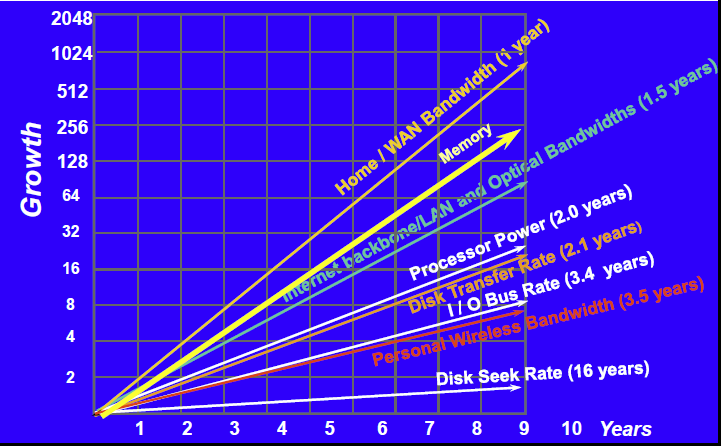
\includegraphics[width=0.9\linewidth]{growth-comparison}

Examples of divergences are:
\begin{itemize}
    \item Processor-Memory performance gap (RAM to slow)
    \item Battery-Computing Power (batteries way to low on capacity)
\end{itemize}

\subsection{Limits of Growth}
The predictions for the future see a limit and a clear end to Moore's Law. It is
very likely that alternative technologies must be explored to further increase
technology power. (i.e. Molecular-, Organic-, Quantum-level and others)

The 5 technical drivers of Ubiquitous Vomputing are:
\begin{description}
    \item[Moore's Law] \ \\
        Increasing computing power and decreasing device size.
    \item[New Materials] \ \\
        e. g. semiconudctors, fibers, flexible substrates (displays etc.),
        E-Ink
    \item[Progress in Communication Technologies] \ \\ 
        Fiber optics, wireless (NFC, RFID, Bluetooth, LTE), opportunistic
        carriers (powerline, body area networks)
    \item[New Architectural and Software Concepts] \ \\
        like Spontaneous Networking (e.g. Universal Plug and Play UPnP)
    \item[Better Sensors] \ \\
        Miniaturized cameras, microphones, biometric sensors, location sensors,
        passive radio frequency (RF) sensors (use piezoelectric and
        pyroelectric materials), RFID 
\end{description}

\section{Radio Frequency Identification (RFID)}
Identify objects from distance to associate specific actions or attributes with
the object or authenticate it. (or a person)

Uses RF-transponder (\underline{Trans}mitter-res\underline{ponder}) and wireless
energy supply by induction or electromagnetic field with range of up to 10 m.
Small amounts of data (up to about 100 bytes) can be stored using ROM (Read
Only Memory) or EEPROM (Electronically Erasable Programmable ROM) and chips are
very cheap and therefore disposable.


Medium range features include collision detection (typically 30 items/s) and
read-write memory (EEPROM, SRAM). High end features are complex functions like
cryptography used in smartcards.

RFID systems are typically classified based on different features:
\begin{itemize}
    \item Power Supply
    \item Operation Frequency
    \item Communication, Coding and Modulation
    \item Anti-Collision Protocols
    \item Memory Structure and Data Access
\end{itemize}

\subsection{Power Supply \& Operation Frequency}
Tag need energy to power microchip and transmit data back to reader. Passive
tags have no internal battery and entirely use energy transmitted by reader
while active RFID tags contain an internal battery which increases range (up to
100m) and lowers environmental influences (no interference with metal, liquids
etc.) while coming at a higher price and bigger size.

There exist two coupling methods for wireless energy supply:
\begin{description}
\item[Inductive Coupling (magnetic field)] \ \\
    Magnetic field generated by reader induces voltage in the coil of the
    transponder. Frequencies typically $100-135 kHz$ (LF) or $13.56 MHz$ (HF).
    Works in the near field for low power usage. Note that EEPROM needs much
    more energy than ROM.
\item[Electromagnetic Coupling] \ \\
    Coupling in the far-field on $868, 915 MHz$ (UHF) and $2.4 Ghz$ (micro
    wave) 
\end{description}

The magnetic {\bf near field} is an energy storage field of strength
$\O(\frac{1}{r^3})$ while the electromagnetic {\bf far field} is an energy
propagating field of strenght $\O(\frac{1}{r})$. The boundary lies at
$\frac{\lambda}{2\pi}$ where their amplitude is equal. Some values are $5$ m at
$10$ MHz and $5$ cm at $1$ GHz. Typically RFID operates in the near field.

\subsection{Communication Principles}
The reader may periodically turn of its field to allow transponders to send
in-between. However this needs a capacitor on transponders to store energy.

\subsubsection{Encoding Schemes}
\begin{description}
\item[NRZ] 1 = high, 0 = low
\item[Manchester Coding] 1 = low-to-high transition, 0 = high-to-low (IEEE
802.3 or reverse for old convention)
\item[Pulse Pause Coding (PPC)] 1 = short period to next pause, 0 = long period
(similar to morse code)
\end{description}

\subsubsection{Data Transfer}
Typically Amplitude Shift Keying (ASK) on the reader's field used to send from
reader to the tag.

From the tag to the reader there are several common principles:
\begin{description}
    \item[Capacitive Coupling] very short distance (mms), electrical field
    \item[Load Modulation] near distance magnetic field, resistor generates
    sub-carrier subject to modulation (ASK, FSK, PSK)
    \item[Backscatter] long range, electromagnetic field, reflection of high
    frequency signal (like radar) with change of reflection properties by
    resistor in parallel to transponder antenna
\end{description}

\subsection{Collision Problem}
Broadcast of reader leads to many simultaneous replies which interfere. While a
transponder typically can't hear signals from other transponders, they still
should have exclusive access to a shared channel during a short period of time.
Therefore collision detection and avoidance have to happen at reader and be
fast and reliable.

\begin{description}
\item[FDMA] \ \\
channels limited, expensive readers, however possible for
small, fixed number of transponder
\item[TDMA] (stochastic) \ \\
{\bf ALOHA} random re-sends $\rightarrow$ bad because optimum
throughput at only $18 \%$ occupation \\
{\bf Slotted ALOHA} maximum throughput $37 \%$ when
only sending at well-defined slots with additional syncing by reader \\
{\bf Adaptive Rounds} Slot count dynamically altered based on load \\
{\bf Reservation ALOHA} Competition phase using ALOHA and phase with reserved
slot transmission (no collision). However causes extra delays
\end{description}

\subsubsection{Capture Effect}
Throughput improves if transponders closer to the reader. They win because of
their stronger signal because a weaker one may not be strong enough to cause
interference. {\bf Weak Collisions} can occur if this leads to collision going
unnoticed.

\subsubsection{Tree Walking Anti-Collision}
With manchester encoding, collisions can be located if two different signals
differ in the same bit. (Leads to illegal high during whole bit period)

\begin{algorithm}[H]
    \SetAlgoLined
    \KwData{Set $T$ with transponders}
    \KwResult{$t \in T$ that can send collision free}
    
    Broadcasts ``sync''\;
    \While{no collision detected}{
        Request ID of all $t \in T$\;
        Determine leftmost bit $b$ that yields a collision\;
        \If{No collision}{
        break\;
        }
        Broadcast ``mute all with $v(b) = 0$''\;
        All $t \in T$ with $v_t(b) = 1$ proceed to next round\;
    }
    Request data from unique $x \in T$\;
    Send ``halt'' to $x$: won't compete until next ``sync''\;
    
    move up tree and repeat\;

    \caption{Tree Walking Cnti-Collision Algorithm}
\end{algorithm}

This is an example of a deterministic TDMA approach (in contrast to the
stochastic ones introduced above)


\subsection{Data Access}
There exist factory programmed read-only tags and read-write tags with a unique
ID plus some additional read-write memory. The latter usually has way worse
performance for writing than reading. In special cases RFID can also be used
with structured memory and access security features.


\subsection{Application-Driven Selection Criteria}
For the needs of a particular application a system is chosen based on the
following criteria:

\begin{description}
\item[Read Range] Antennas, environment, data rate, frequency and transmission
power; whereas the latter 3 typically are regulated and standardized.
\item[Data Transfer and Detection Rates] Low and High Frequency about $5$ kb/s
and UHF $50$ kb/s. Detection rate (time to identify tag) depends on transfer
rate, length of tag ID, anti-collision algorithm (typically between 20 (LF,HF)
and 300 (UHF) tags per second)
\item[Suspectivility to Noise and other Error Sources] Interference, collisions,
absorption, tag misalignment and detuning
\item[Cost] depends on size and complexity of chip; production volume and
technology; antennas and assembly
\item[Tag Form Factors] Size and form
\end{description}

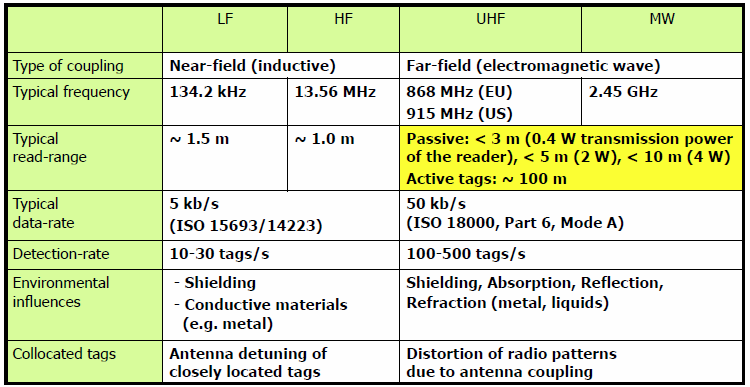
\includegraphics[width=0.9\linewidth]{rfid-properties-overview}

\subsection{RFID vs. Barcodes}
No line of sight required, longer identification range, more data, (nearly)
simultaneous reading, write and delete access, fraud difficult. However comes at
higher cost and is unreliable under certain conditions.

\subsection{RFID Future}
Highest potential currently seen in retail ($10000$ billion \$ per year), postal
services ($650$), books $50$ and drugs $30$. RFID is subject to continuous
adoptions due to Government regulations (e.g. animal identification, biometric
passports), industry leaders adopting their standards, and cost of RFID
equipment.

\subsubsection{Electronic Product Code}
To identify single object instances rather than whole object classes. Decouple
identity from data and only store the EPC on the RFID tag and all additional
information in external databases. The goal is to replace the wide spread
13-digit EAN 13 bar codes (European Article Number) with 96 bit EPC RFID tags.

Standardized interfaces and data formats enable cross enterprise business
processes and decentralized information sharing.

{\bf Object Name Service} (ONS) is used to resolve EPC to URI where the URI
points to something that provides more information on the product or that
triggers an operation (e.g. web page, EPC information service, WSDL to
webservice)

\subsection{Reception in Public}
Many concerns about privacy and infrastructure. Solutions include kill-feature
(deactivate tags at sales point) but this often doesn't satisfy skeptical
customers, vendors might want after-sales services and manufaturers want to add
additional product functionality.

RFID Kill stations can only change the writable part of the memory and the
manufacturer's unique ID in the ROM is not ``killable''.

\subsubsection{Infrastructure Concerns}
Include security of data and controlling access, interoperability between
various solutions, access to historical data (not only processing current
events), cost and complexity of managing, policy issues and more.

\subsection{Applications}
\begin{description}
    \item[Electronic Articel Surveillance (EAS)] Products in super market
    (first introduced in 1966)
    \item[Ski Ticketing]
    \item[Debit System, Wireless Payment]
    \item[Car Immobilizer] (Anti-Theft device)
    \item[Automatic Toll Collection]
    \item[E-Ticket and E-Passports]
    \item[Logistics] Real time inventory and product tracking
\end{description}


\section{Smart Cards}
Portable and secure container for secret data providing a secure execution
environment for cryptographic algorithms. Used e. g. in mobile phone subscriber
information (SIM), credit and debit cards, public telephony, healthcare and
enterprise security (encryption etc.).

\begin{description}
\item[Memory Cards] Cheap ($< 1 €$) but not smart, container for data (usually
with PIN access control for parts of the memory), low level of security for use
in prepaid cards, loyalty cards and disposable applications
\item[Processor Cards] True ``smart cards'' with internal microprocessor and RAM
to perform internal calculations so secret data never leaves card (e.g. private
key). Can contain true random generator but has much higher price. Typically up
to 256 kB ROM and 128 kB EEPROM.
\end{description}

\subsection{Random Number Generation}
Pseudo random number is generate based on some logical CPU states (e.g.
registers) that are incremented by a clock or a crypto algorithm such as DES.

True random number generator can be in hardware and exploit physical
characteristics with varying performance depending on how long it takes to build
up a sufficient level of entropy.

\subsection{Communication}
Communication is initiated by the reader (terminal) as client with the card as
server. The communication protocol is half-duplex with typically 9.6 kbit/s (up
to 115) and either byte- or block-oriented. Newer generations of smart cards
communicate via the USB protocol using two originally unused connections on the
chip. This allows speeds of up to 1.5 Mbit/s full duplex.


\subsection{Smart Card System}
Simple and small ($3-30$ kB) {\bf Operating System} without user interface,
interrupts or multiprogramming. Highly dependent on the hardware and primarily optimized
for security. Offers API to operating system functions like access to file
system, cryptographic functions and I/O. Most important OSes are {\it JavaCard}
and {\it MULTOS}.

The {\bf File System} is held as a tree in EEPROM allowing different types of
files (e.g. fixed vs. variable sized records) and access control. There exist
several file access commands for creation, deletion, writing, reading,
appending, locking, invalidating and seeking that can then be performed on the
card without further request-reply cycles with the client.

\subsubsection{JavaCard}
JavaCard is a stripped down Java VM on the card which is directly programmable
in Java (subset: no threads, cloning, strings, large data types or dynamic
class loading) and offers a standardized interface to the card (Java Card API).
Applets can be loaded dynamically into the card.

This allows for very easy application development on a high level and increased
flexibility because the software can be loaded/replaced at any time. A major
disadvantage is however the worse performance, as the execution time is about
four times slower than for native code.

Multiple applets are prohibited from interaction with each other by a applet
firewall to guarantee security. Only the terminal can select applets to be
loaded for execution.

\subsection{Subscriber Identity Module (SIM)}
SIM is a security module for accessing mobile phone networks to enable
separation of phone and service marketing. It is currently the largest market
for smart cards and the execution platform for mobile applications.

Used to store unique {\bf International Mobile Subscriber Identity} (IMSI),
encryption key, current location, service provider, preferred language and other
relevant information.

\subsection{Contact-less Smart Cards}
As described in ISO 14443, smart cards using external energy sources similar to
RFID with the capability for contact-less interaction do exist. They have a
range of a few centimeters, are more expensive and provide improved security
compared to RFID tags because they have direct cryptography support.


\subsection{Security Issues}
With direct hardware access no such thing as $100 \%$ security exists. However
the price/protection ratio must be considered. While smart cards are relatively
secure due to support for terminal, card and user authentication, the right
tools can help in breaching security and gaining access to stored data.

This can be achieved by reverse engineering the logic circuits or the ROM
content using microscopes and similar equipment. It is even possible to set bits
with UV pulses of X rays to specific memory locations. A possible use could be
to manipulate the random generator to always yield the same number or manipulate
the DES algorithm.

Simple attacks include forcing glitches by clock bursts (rapid increase in
clock frequency) or voltage glitches to learn secret keys or bypass security
checks. More sophisticated attacks try to retrieve keys by side-channel
information like power consumption, heat and timing during encryption. This type
of attacks is applicable for almost all crypto algorithms and smart cards with
simple requirements of a digital oscilloscope, a smart card reader and a PC.

\subsubsection{Countermeasures}

There exist {\bf hardware} countermeasures to power and timing analysis like
reducing and balancing power consumption, increasing noise, vary execution time
of instructions and randomly modifying internal clock speed. {\bf Software}
countermeasures include adding random instructions to desynchronize, limit
number of executions for algorithm and the elimination of all correlation
between timing and data or key.

In general this includes scrambling of the data bus and memory cells, checksums
on memory contents, encryption of memory content, redundant computing and bus
data and the use of dual logic. (10 = low, 01 = high $\rightarrow$ always uses the same amount of
power) {\bf Active Shielding} uses sensors (e.g. reacting to light or increased
clock rate, i. e. temperature) and performance analysis to detect a potential
attack. If an attack is detected, critical parts of the EEPROM can be
overwritten.

\section[Wireless short-distance communication]{Wireless short-distance
communication%
\footnote{For more detailed information about wireless network basics and the
Bluetooth protocol please consult~\cite{acn-summary}.}
}

\subsection{Comparison to fixed Networks}
Wireless networks typically have way higher loss rates due to interference,
fading etc. and are restricted to regulations of resources (frequency bands).
They typically achieve lower transmission rates and are less secure due to the
publicly shared transmission medium. However they have great mobility support
and need less infrastructure.

Major challenges of mobility include varying transmission quality, disconnection
management, handover, location transparency, service discovery,
authentication and security.

\subsection{Multiplexing}
There are four basic multiplexing methods that are usually combined to achieve a
real-world compatible solution:
\begin{itemize}
    \item Space Division Multiplexing Access
    \item Frequency Division Multiplexing Access
    \item Time Division Multiplexing Access
    \item Code Division Multiplexing Access
\end{itemize}

In FDMA two versions are commonly distinguished: Fast and Slow Hopping. While in
{\bf Fast Hopping} several frequencies per bit are used, {\bf Slow Hopping}
sends several bits per frequency.

An example of the combination of TDMA and FDMA is the widely used GSM protocol
for mobile phones.

\subsection{Bluetooth}
Bluetooth 802.15.1 is for short-range (typically up to $10$m) medium bandwidth
($< 1$ Mb/s) data transfers in spontaneously created small networks. It operates
in the $2.4$ GHz frequency band on $79$ channels with $1600$ frequency hops per
second ($625 \mu$s intervals).

Two basic modes (baseband link types) exist: One for synchronous, timing
critical transmission like voice and one for asynchronous transmissions like data.

Bluetooth devices can form a so called piconet of up to 8 devices with 1 master
that determines clock and frequency hopping pattern (based on its device ID).
All communication always goes over the master, there is no possibility for
direct slave-to-slave communication. Because a slave can participate in multiple
piconets at once (but at most in one actively at any time) it is possible to
form scatternets of multiple overlapping piconets where slaves in multiple
piconets serve as bridges.

The further development of the Bluetooth standards (currently version 3.0) tries
to achieve higher data rates with lower power consumption for a cheaper price.
Since Bluetooth 2.1 (2007) pairing between devices became much simpler and with
Bluetooth 3.0 (2009) WiFi can be used on the physical layer to enable for much
higher transfer rates.

\subsection{802.15.4}
For even smaller, cheaper and less energy consuming communication devices like
smart watches, remote controls or sensor networks, IEEE 802.15.4 provides a
suitable solution. It is designed to allow building multi-month (or even year)
battery life personal area networks with support for latency-critical
applications. Nodes can operate in a master-slave fashion or peer-to-peer in
mesh networks and transfer data with up to $250$ kbit/s. The standard only
defines the physical and MAC layer.


{\bf ZigBee} is an upper layer protocol based in IEEE 802.15.4 that defines the
network and application layer and implements mesh topologies using multi-hop and
ad hoc on-demand distance vector
routing.%
\footnote{\href{http://en.wikipedia.org/wiki/Distance-vector_routing_protocol}
{http://en.wikipedia.org/wiki/Distance-vector\_routing\_protocol}}


{\bf 6LoWPAN} (IPv6 over Low-Power Wireless Personal Area Networks) sends IPv6
packets over 802.15.4 using aditional header compression and packet
fragmentation. It supports both mesh-under (link layer) and route-over (IP
layer) routing.

\subsection{Near Field Communication (NFC)}

\bibliographystyle{plain}
\bibliography{references}

\clearpage
\end{multicols}
\end{document}
